% pyformex manual --- tutorial
% $Id$
% (C) B.Verhegghe

\chapter{pyFormex tutorial}
{\label{cha:tutorial}


%%
\section{Introduction}
\label{sec:intro-tut}

\pyformex is a Python implementation of Formex algebra. Using \pyformex, it is very easy to  generate large geometrical models of 3D structures by a sequence of mathematical transformations. It is especially suited for the automated design of spatial frame structures. But it can also be used for other tasks, like finite element preprocessing, or just for creating some nice pictures.

By writing a very simple script, a large geometry can be created by copying, translating, rotating,... Formices. \pyformex will interpret this script and draw what you have created. This is clearly very different than the traditional way of creating a model, like CAD. There are two huge advantages about using \pyformex:
\begin{itemize}
\item It is especially suited for the automated design of spatial frame structures. A dome, arc, hypar,... can be rather difficult to draw with CAD, but when using mathematical transformations, it becomes a piece of cake!
\item Using a script makes it very easy to apply changes in the geometry: you simply modify the script and let \pyformex play it again. For instance, you can easily change an angle, the radius of a dome, the ratio $f/l$ of an arc,... Using CAD, you would have to make an entirely new drawing! This is also illustrated in figure~\ref{fig:scallops}: these domes were all created with the same script, but with other values of the parameters.
\end{itemize}
\begin{figure}[h]
  \centering
  \begin{makeimage}
  \end{makeimage}
  \begin{latexonly}
    \subfigure[A basic Scallopdome]{\label{scallop}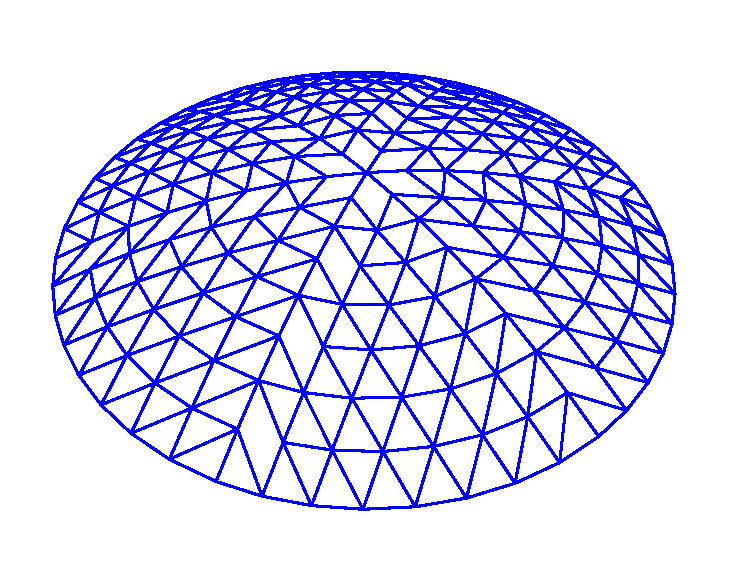
\includegraphics[width=5cm]{images/scallopdome-000}}
    \hfill
    \subfigure[Another Scallopdome]{\label{scallop2}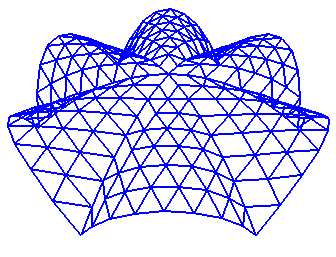
\includegraphics[width=5cm]{images/scallopdome-001}}
    \hfill
    \subfigure[Yet another Scallopdome]{\label{scallop3}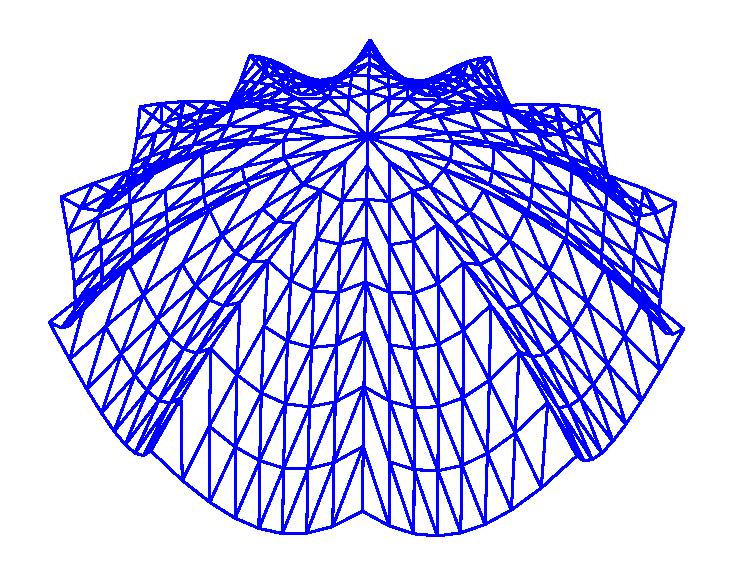
\includegraphics[width=5cm]{images/scallopdome-002}}
  \end{latexonly}
  \begin{htmlonly}
%    \htmladdimg[WIDTH="300"]{../images/scallopdome-000.png}
    \htmladdimg{../images/scallopdome-000.png}
    \htmladdimg{../images/scallopdome-001.png}
    \htmladdimg{../images/scallopdome-002.png}
  \end{htmlonly}
  \caption{Same script, different domes} \label{fig:scallops}
\end{figure}

% As mentioned, \pyformex is based on the programming language Python \footnote{\url{http://www.python.org}}. This implies that the scripts are also Python-based. It's a very easy language, but if you're interested in reading more, there is a very good tutorial available on \url{http://docs.python.org/tut/}. However, if you're only using Python to write \pyformex-scripts, the tutorial you're reading right now should be enough. 


%%%%%%%%%%%%%%%%%%%%%%%%%%%%%%%%%%%%%%%%%%%%%%%%%%%%%%%%%%%%%%%%%%%
\section{Getting started}
\label{sec:getting-started}


THis i the first paragrph.

This section holds some basic information on how to use Python and \pyformex. 

\begin{itemize}
\item Each script should begin with \Code{\#!/usr/bin/env pyformex}
\item To start the \pyformex GUI, double click on the file \file{pyformex} in the installation directory, or type \emph{pyformex} in the terminal. Using the terminal can be very useful, because errors that are created while running the script will appear in the terminal. This can provide useful information when something goes wrong with your script.
\item To create a new \pyformex-script, just open a new file with your favorite text editor and save it as \file{myproject.py}.
\item To edit a script, you can
	\begin{itemize}
	\item Open it with your favorite text editor.
	\item \menuselection{File \sub Open}\\
	At this point, the script will be loaded but nothing will happen. \\
	\menuselection{File \sub Edit}\\
	The script will now open in the default text editor. This default editor can be changed in the file \file{.pyformexrc} in 		the installation directory.
	\end{itemize}
\item To play a script, you can
	\begin{itemize}
	\item \menuselection{File \sub Open}\\
		\menuselection{File \sub Play} 
	\item Type \emph{pyformex myproject.py} in the terminal. This will start the \pyformex GUI and load your script at the same time. \\
\menuselection{File \sub Play}
	\item To play a script without using the GUI (for example in finite element preprocessing, if you only want to write an 		output file, without drawing the structure), type \emph{pyformex --nogui myproject.py}
	\end{itemize}
\item When writing a script in Python, there are some things you should keep in mind:
	\begin{itemize}
	\item When using a function that requires arguments, an argument list must have any positional arguments followed by any keyword arguments, where the keywords must be chosen from the formal parameter names. It's not important whether a formal parameter has a default value or not. No argument may receive a value more than once -- formal parameter names corresponding to positional arguments cannot be used as keywords in the same calls. 

Simply put: you can either set the arguments in the right order and only give their value, or you can give arguments by their name and value. This last option holds some advantages: not only is it easier to check what you did, but sometimes a function has many arguments with default values and you only want to change a few.
If this isn't entirely clear yet, just look at the examples later in this tutorial or check the Python tutorial.
	\item Indentation is essential in Python. Indentation is Python's way of grouping statements. In straight-forward scripts, indentation is not needed (and forbidden!), but when using a for-statement for example, the body of the statement has to be indented. A small example might make this clear. Also notice the ':' 
\begin{verbatim}
	print 'properties'
	for key, item in properties.iteritems():
	    print key, item
\end{verbatim}
	\item If you want to use functions from a seperate module (like \module{properties}), you add a line on top of the script
\begin{verbatim}
	from properties import *
\end{verbatim}
All functions from that module are now available.
	\item The hash character, "\#", is used to start a comment in Python.
	\item Python is case sensative.
	\end{itemize}
\end{itemize}


%%%%%%%%%%%%%%%%%%%%%%%%%%%%%%%%%%%%%%%%%%%%%%%%%%%%%%%%%%%%%%%%%
\section{The geometrical model}
\label{sec:geom}


\subsection{Creating a Formex}
\label{subsec:create}

\subsubsection{What is a Formex?}
A Formex\index{Formex} is a numarray of order 3 (axes 0,1,2) and type Float.
A scalar element represents a coordinate (F:uniple).

    A row along the axis 2 is a set of coordinates and represents a point
    (node, vertex, F: signet).
    For simplicity's sake, the current implementation only deals with points
    in a 3-dimensional space. This means that the length of axis 2 is always 3.
    The user can create Formices (plural of Formex) in a 2-D space, but
    internally these will be stored with 3 coordinates, by adding a third
    value 0. All operations work with 3-D coordinate sets. However, a method
    exists to extract only a limited set of coordinates from the results,
    permitting to return to a 2-D environment.

    A plane along the axes 2 and 1 is a set of points (F: cantle). This can be
    thought of as a geometrical shape (2 points form a line segment, 3 points
    make a triangle, ...) or as an element in FE terms. But it really is up to
    the user as to how this set of points is to be interpreted.

    Finally, the whole Formex represents a set of such elements.

    Additionally, a Formex may have a property set, which is an 1-D array of
    integers. The length of the array is equal to the length of axis 0 of the
    Formex data (i.e. the number of elements in the Formex). Thus, a single
    integer value may be attributed to each element. It is up to the user to
    define the use of this integer (e.g. it could be an index in a table of
    element property records).
    If a property set is defined, it will be copied together with the Formex
    data whenever copies of the Formex (or parts thereof) are made.
    Properties can be specified at creation time, and they can be set,
    modified or deleted at any time. Of course, the properties that are
    copied in an operation are those that exist at the time of performing
    the operation.   

Simply put: a Formex is a set of elements, and every element can have a property number.
\begin{figure}[h]
  \centering
  \begin{makeimage}
  \end{makeimage}
  \begin{latexonly}
    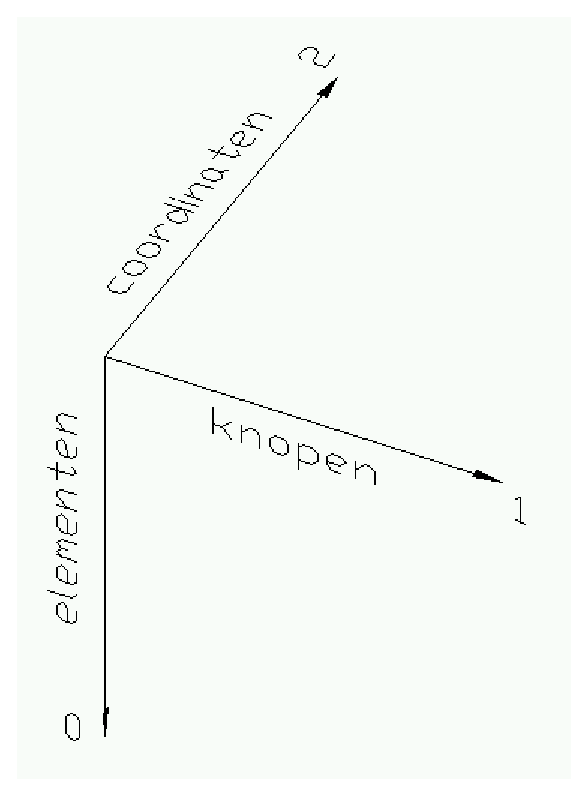
\includegraphics[width=4cm]{images/Formex}
  \end{latexonly}
  \begin{htmlonly}
    \htmladdimg{../images/Formex.png}
  \end{htmlonly}  
  \caption{The scheme of a Formex}
\end{figure}

\subsubsection{Creating a Formex using coordinates}
The first and most useful way to create a Formex is by specifying it's nodes and elements in a 3D-list.  

\begin{verbatim}
	F=Formex([[[0,0],[1,0],[1,1],[0,1]]])
\end{verbatim}

\begin{figure}[h]
  \centering
  \begin{makeimage}
  \end{makeimage}
  \begin{latexonly}
    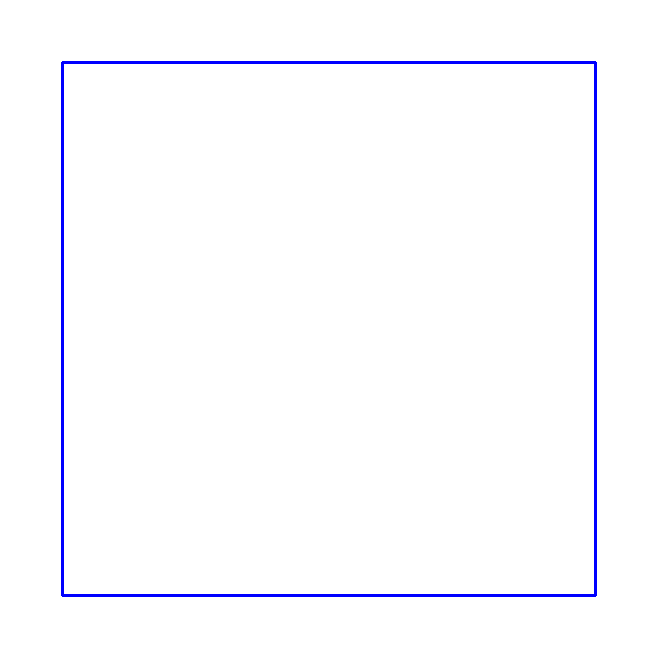
\includegraphics[width=4cm]{images/square}
  \end{latexonly}
  \begin{htmlonly}
    \htmladdimg{../images/square.png}
  \end{htmlonly}  
  \caption{A very simple Formex}
  \label{fig:square}
\end{figure}

This creates a Formex F, which has the nodes (0,0), (1,0), (1,1) and (0,1). These nodes are all part of a single element, thus creating a square plane. This element is also the entire Formex.
On the other hand, if you would change the position of the square brackets like in the following example, then you'd create a Formex F which is different from the previous. The nodes are the same, but the connection is different. The nodes (0,0) and (1,0) are linked together by an element, and so are the nodes (1,1) and (0,1). The Formex is now a set of 2 parallel bars, instead of a single square plane. 
\begin{verbatim}
	F=Formex([[[0,0],[1,0]],[[1,1],[0,1]]])
\end{verbatim}

\begin{figure}[h]
  \centering
  \begin{makeimage}
  \end{makeimage}
  \begin{latexonly}
    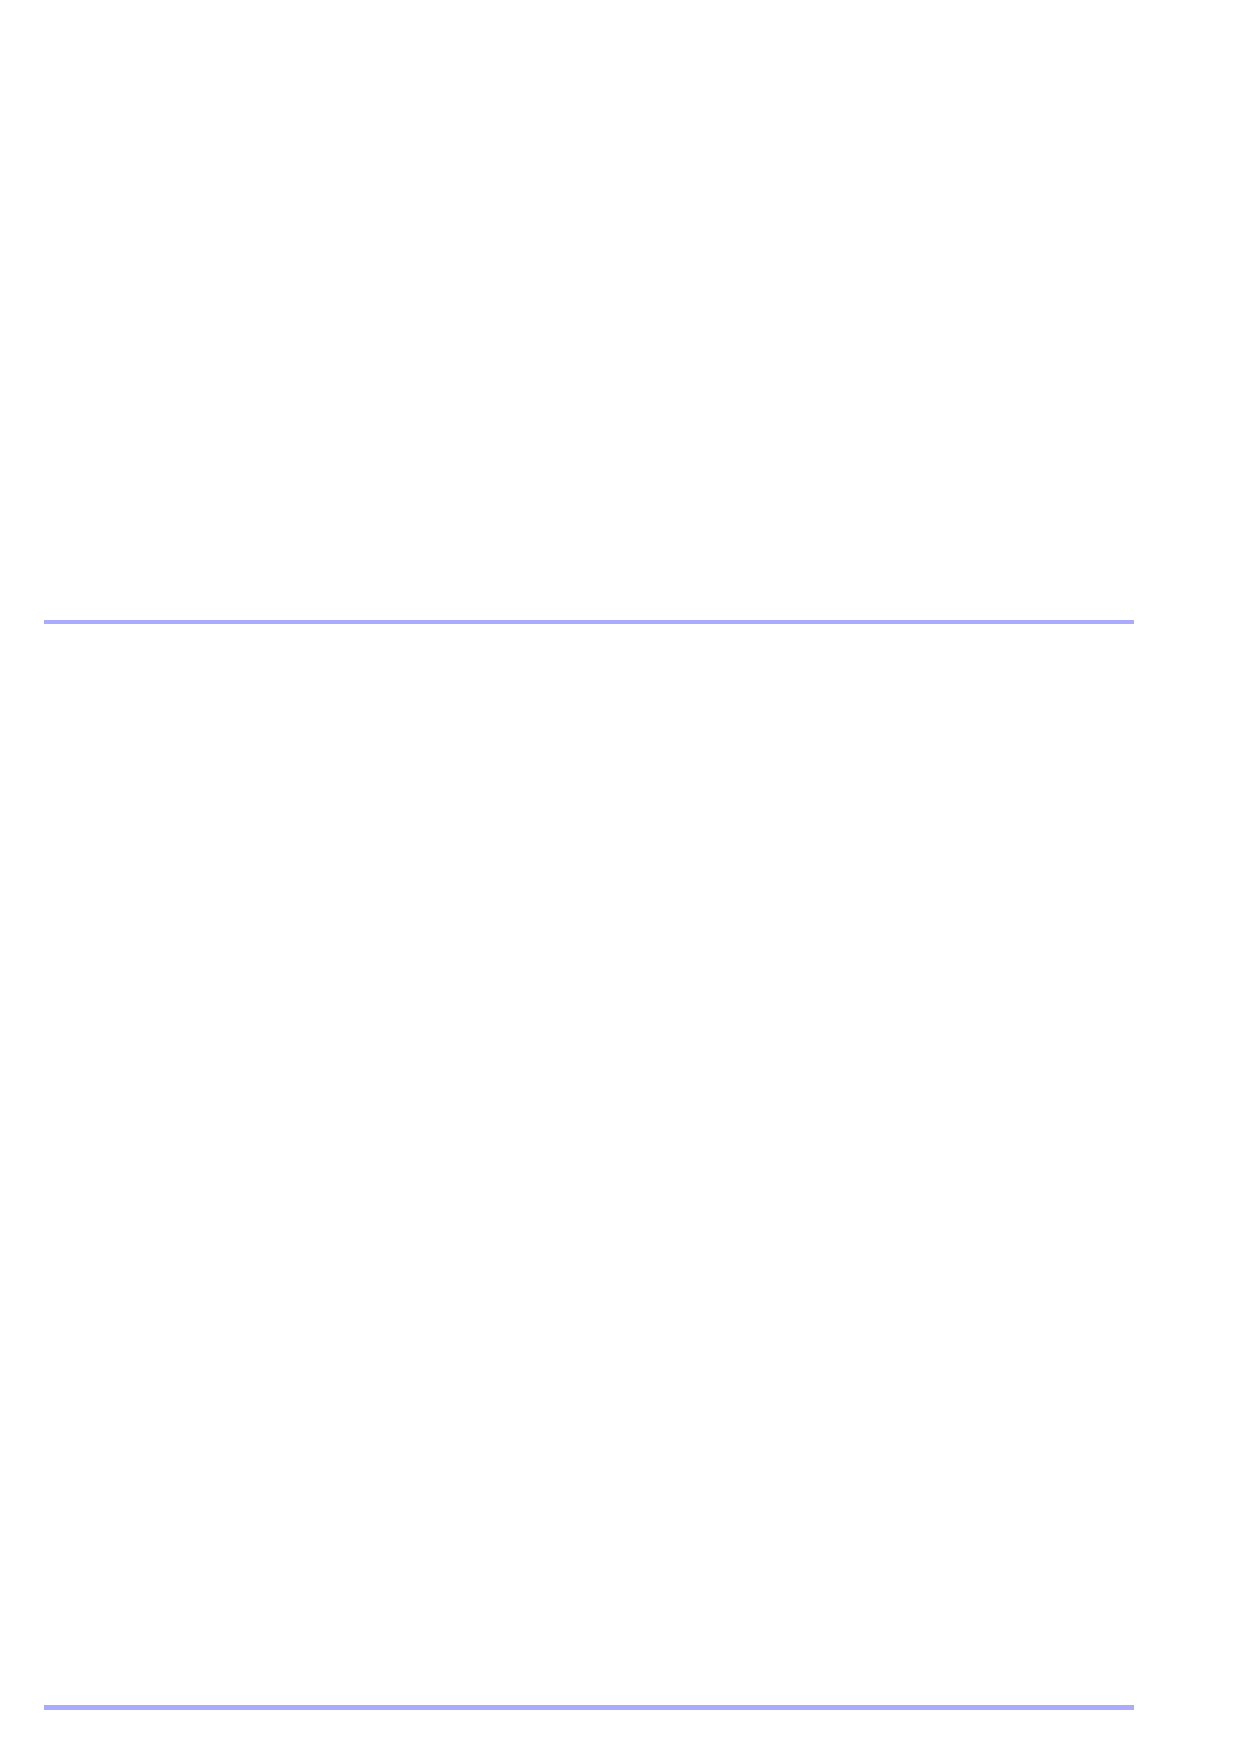
\includegraphics[width=4cm]{images/parallel}
  \end{latexonly}
  \begin{htmlonly}
    \htmladdimg{../images/parallel.png}
  \end{htmlonly}  
  \caption{Same nodes, different Formex}
\end{figure}

If we want to define a Formex, similar to the square plane, but consisting of the 4 edges instead of the actual plane, we have to define four elements and combine them in a Formex. This is \emph{not} the same Formex as fig \ref{fig:square}, although it looks exactly the same.
\begin{verbatim}
	F=Formex([[[0,0],[0,1]], [[0,1],[1,1]], [[1,1],[1,0]], [[1,0],[0,0]]])
\end{verbatim}

The previous examples were limited to a 2-D environment for simplicity's sake. Of course, we could add a third dimension. For instance, it's no problem defining a pyramid consisting of 8 elements ('bars').
\begin{verbatim}
	F=Formex([[[0,0,0],[0,1,0]], [[0,1,0],[1,1,0]], [[1,1,0],[1,0,0]], [[1,0,0], 
		[0,0,0]], [[0,0,0],[0,1,0]], [[0,0,0],[0.5,0.5,1]], [[1,0,0],[0.5,0.5,1]], 
		[[1,1,0], [0.5,0.5,1]], [[0,1,0],[0.5,0.5,1]]])
\end{verbatim}

\begin{figure}[h]
  \centering
  \begin{makeimage}
  \end{makeimage}
  \begin{latexonly}
    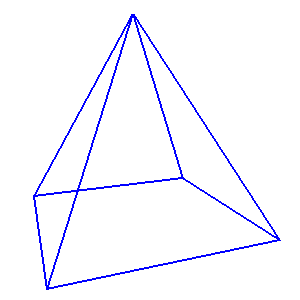
\includegraphics[width=6cm]{images/pyramide}
  \end{latexonly}
  \begin{htmlonly}
    \htmladdimg{../images/pyramide.png}
  \end{htmlonly}  
  \caption{A pyramid}
  \label{fig:pyramid}
\end{figure}

However, as you can see, even in this very small example the number of nodes, elements and coordinates you have to declare becomes rather large. Defining large Formices using this method would not be practical. This problem is easily overcome by copying, translating, rotating,... a smaller Formex --- as will be explained in \ref{subsec:changing} --- or by using patterns.
 
\subsubsection{Creating a Formex using patterns}

The second way of creating a new Formex, is by defining patterns. In this case, a line segment pattern is created from a string.

The function \function{pattern(s)} creates a list of line segments where all nodes lie on the
gridpoints of a regular grid with unit step.
The first point of the list is [0,0,0]. Each character from the given
string \var{s} is interpreted as a code specifying how to move to the next node.
Currently defined are the following codes:\\
    0 = goto origin [0,0,0]\\
    1..8 move in the x,y plane\\
    9 remains at the same place\\
    When looking at the plane with the x-axis to the right,\\
    1 = East, 2 = North, 3 = West, 4 = South, 5 = NE, 6 = NW, 7 = SW, 8 = SE.\\
    Adding 16 to the ordinal of the character causes an extra move of +1 in
    the z-direction. Adding 48 causes an extra move of -1. This means that
    'ABCDEFGHI', resp. 'abcdefghi', correspond with '123456789' with an extra
    z +/-= 1.              
    The special character '\verb?\?' can be put before any character to make the
    move without making a connection.
    The effect of any other character is undefined.

This method has important restrictions, since it can only create lines on a regular grid. However, it can be a much easier and shorter way to define a simple Formex. This is illustrated by the difference in length between the previous creation of a square and the next one, although they define the same Formex (figure \ref{fig:square}).
\begin{verbatim}
	F=Formex(pattern('1234'))
\end{verbatim}

Some simple patterns are defined in \module{simple.py} and are ready for use. These patterns are stacked in a dictionary called 'Patterns'. Items of this dictionary can be accessed like \Code{Patterns['cube']}.
\begin{verbatim}
	#!/usr/bin/env pyformex
	from simple import *
	c=Formex(pattern(Pattern['cube']))
	clear();draw(c)
\end{verbatim}

\begin{figure}[h]
  \centering
  \begin{makeimage}
  \end{makeimage}
  \begin{latexonly}
    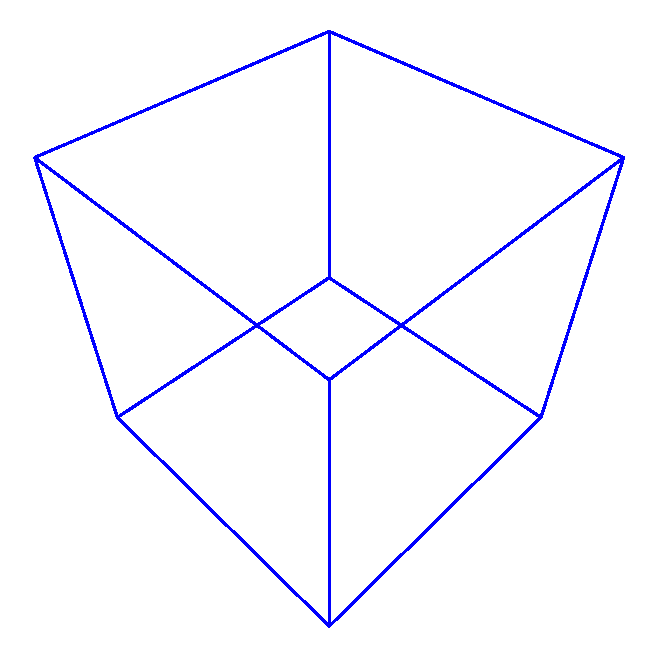
\includegraphics[width=6cm]{images/cube}
  \end{latexonly}
  \begin{htmlonly}
    \htmladdimg{../images/cube.png}
  \end{htmlonly}  
  \caption{A cube}
  \label{fig:cube}
\end{figure}

\subsubsection{Creating a Formex using coordinates from a file}
In some cases, you might want to read coordinates from a file an combine them into a Formex. This is possible with the module \module{file2formex} and it's function \function{fileFormex()}. Each point is connected to the following, forming an element (bar).

The next file ('square.txt') would create the same square as before(figure \ref{fig:square}).
\begin{verbatim}
	0,0,0
	0,1,0
	1,1,0
	1,0,0
\end{verbatim}
\begin{verbatim}
	#!/usr/bin/env pyformex
	from file2formex import *
	F=fileFormex('square.text', closed='yes')
\end{verbatim}

\subsection{Adding property numbers}
\label{subsec:propnr}
Each Formex element can have a property number. Each property number is represented by a different color when the Formex is drawn. This is the first reason why you could use property numbers: to make your drawing more transparent or just more beautiful. However, these numbers can also be used as an entry in a dictionary of properties - thus linking the element with a property. This property can be about anything, but in finite element processing this would be the element section, material, loads,... The use of properties in this way will be futher explained in \ref{sec:props}.
Property numbers can be specified at creation time, and they can be set, modified or deleted at any time.  
\begin{verbatim}
>>> #!/usr/bin/env pyformex
>>> F=Formex(pattern('1234'),[5])
>>> print F.prop()
>>> G=Formex(pattern('1234'),[6,8,2,4])
>>> print G.prop()
>>> F.setProp([6,7])
>>> print F.prop()
>>> G.setProp([6,7,8,9])
>>> print G.prop()

[5 5 5 5]
[6 8 2 4]
[6 7 6 7]
[6 7 8 9]
\end{verbatim}

\subsection{Drawing a Formex}
\label{subsec:drawing}
Of course, you'd want to see what you have created. This is accomplished by the function \function{draw()}. The next example creates figure \ref{fig:pyramid}. 
\begin{verbatim}
	F=Formex([[[0,0,0],[0,1,0]], [[0,1,0],[1,1,0]], [[1,1,0],[1,0,0]], [[1,0,0], 
		[0,0,0]], [[0,0,0],[0,1,0]], [[0,0,0],[0.5,0.5,1]], [[1,0,0],[0.5,0.5,1]], 
		[[1,1,0], [0.5,0.5,1]], [[0,1,0],[0.5,0.5,1]]])
	draw(F)
\end{verbatim}

It also possible to draw multiple Formices at the same time.
\begin{verbatim}
	from simple import *
	F=Formex([[[0,0,0],[0,1,0]], [[0,1,0],[1,1,0]], [[1,1,0],[1,0,0]], [[1,0,0],
		[0,0,0]], [[0,0,0],[0,1,0]], [[0,0,0],[0.5,0.5,1]], [[1,0,0],[0.5,0.5,1]], 
		[[1,1,0],[0.5,0.5,1]], [[0,1,0],[0.5,0.5,1]]]).setProp(1)	
	G=Formex(pattern(Pattern['cube'])).setProp(3)
	draw(F+G)
\end{verbatim}
\begin{figure}[h]
  \centering
  \begin{makeimage}
  \end{makeimage}
  \begin{latexonly}
    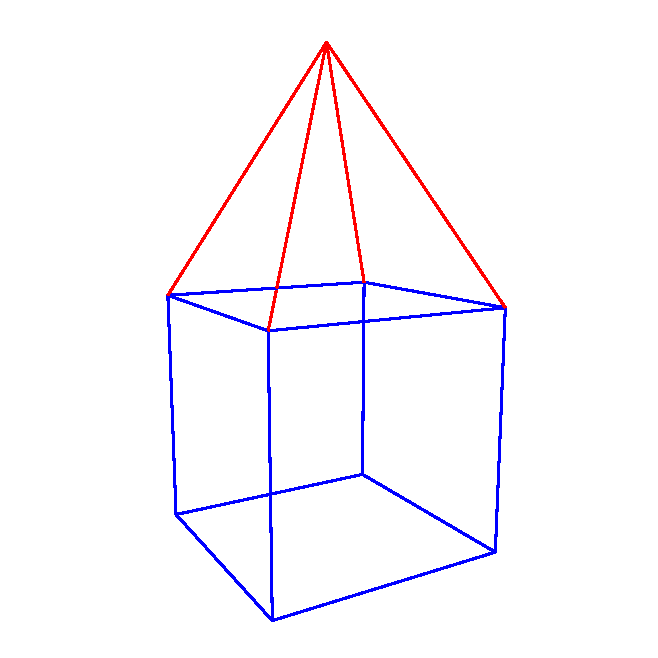
\includegraphics[width=6cm]{images/house}
  \end{latexonly}
  \begin{htmlonly}
    \htmladdimg{../images/house.png}
  \end{htmlonly}  
  \caption{Drawing multiple Formices}
  \label{fig:multiple}
\end{figure}
 
It might be important to realize that even if you don't draw a particular Formex, that doesn't mean you didn't create it!

Now, when you are creating a large geometry, you might be interested in seeing the different steps in the creation. To remove all previously drawn Formices, you can use \function{clear()}  what sweepes the screen clean. If you want to see a certain step in the creation longer than the default time, use \function{sleep(t)}, with \var{t} the delay (in seconds) before executing the next command.
\begin{verbatim}
	F=Formex(pattern('164'))
	draw(F)
	G=F.replic(5,1,0)
	clear()
	draw(G)
\end{verbatim}


\subsection{Saving images}
\label{subsec:images}
After drawing the Formex, you might want to save the image. This is very easy to do:\\
\menuselection{File \sub Save Image}\\
The filetype should be 'bmp', 'jpg', 'pbm', 'png', 'ppm', 'xbm', 'xpm', 'eps', 'ps', 'pdf' or 'tex'. \\
To create a better looking picture, several settings can be changed:
\begin{itemize}
	\item Change the background color \menuselection{Settings \sub Background Color}
	\item Use a different (bigger) linewidth \menuselection{Settings \sub Linewidth}
	\item Change the canvas size. This prevents having to cut and rescale the figure with an image manipulation program (and loosing quality by doing so).  \menuselection{Settings \sub Canvas Size}
\end{itemize}

It is also possible to save a series of images. This can be especially useful when playing a script which creates several images, and you would like to save them all.  For example, figure \ref{fig:WireStent steps}, which shows the different steps in the creation of the WireStent model, was created this way.\\
\menuselection{File \sub Toggle MultiSave}\\


\subsection{Information about a Formex}
\label{subsec:info}
There are a number of functions available that return information about a Formex. Especially when using \pyformex as finite element preprocessor, the most useful functions are:
\begin{tableii}{l|l}{exception}{Function}{Description}
	\lineii{F.nelems()			}
		{Return the number of elements in the Formex.}
	\lineii{F.nnodes() 			}
		{Return the number of nodes in the Formex.}
	\lineii{F.prop() 				}
		{Return the properties as a numpy array.}
	\lineii{F.bbox()				}
		{Return the bounding box of the Formex.}
	\lineii{F.center()			}
		{Return the center of the Formex.}
	\lineii{F.feModel()	}
		{Return a tuple of nodal coordinates and element connectivity.}
\end{tableii}

\function{feModel()} is very important in finite element processing. It returns all nodes and all elements of the Formex in a format useful for FE processing. A tuple of two arrays is returned. The first is float array with the coordinates of the unique nodes of the Formex. The second is an integer array with the node numbers connected by each element.
\begin{verbatim}
>>> #!/usr/bin/env pyformex
>>> from simple import *

>>> c = Formex(pattern(Pattern['cube']))
>>> draw(c)
>>> nodes,elems = c.feModel()
>>> print 'Nodes'
>>> print nodes
>>> print 'Elements'
>>> print elems

Nodes
[[ 0.  0. -1.]
 [ 1.  0. -1.]
 [ 0.  1. -1.]
 [ 1.  1. -1.]
 [ 0.  0.  0.]
 [ 1.  0.  0.]
 [ 0.  1.  0.]
 [ 1.  1.  0.]]
Elements
[[4 5]
 [5 7]
 [7 6]
 [6 4]
 [4 0]
 [5 1]
 [7 3]
 [6 2]
 [0 1]
 [1 3]
 [3 2]
 [2 0]]
\end{verbatim}

\subsection{Changing the Formex}
\label{subsec:changing}
Until now, we've only created simple Formices. The strength of \pyformex however is that it is very easy to generate large geometrical models by a sequence of mathematical transformations. After initiating a basic Formex, it's possible to transform it by using copies, translations, rotations, projections,...

There are many transformations available, but this is not the right place to describe them all. This is what the reference manual in chapter \ref{cha:reference} is for. A summary of all possible transformations and functions can be found there.

To illustrate some of these transformations and the recommended way of writing a script, we will analyse some of the examples. More of these interesting examples are found in \file{installdir/examples}. Let's begin with the example \file{Spiral.py}. 

\verbatiminput{scripts/Spiral.py}

During this first read-through, you will have noticed that every step is drawn. Of course, this is not necessary, but it can be useful. And above all, it is very educational for use in a tutorial...

The next important thing is that parameters were used. It's recommended to always do this, especially when you want to do a parametric study of course, but it can also be very convenient if at some point you want to change the geometry (for example when you want to re-use the script for another application).

A simple function \function{drawit()} is defined for use in this script only. This function only provides a shorter way of drawing Formices, since it combines \function{clear()} and \function{draw}. 

Now, let's dissect the script.

\begin{verbatim}
def drawit(F,view='front'):
    clear()
    draw(F,view)
\end{verbatim}
This is a small function that is only defined in this script. It clears the screen and draws the Formex at the same time. 

\begin{verbatim}
m = 36 # number of cells along torus big circle
n = 10 # number of cells along torus small circle
\end{verbatim}
These are the parameters. They can easily be changed, and a whole new spiral will be created without any extra effort.
The first step is to create a basic Formex. In this case, it's a triangle which has a different property number for every edge.
\begin{verbatim}
F = Formex(pattern("164"),[1,2,3]); drawit(F)  
\end{verbatim}
\begin{figure}[h]
  \centering
  \begin{makeimage}
  \end{makeimage}
  \begin{latexonly}
    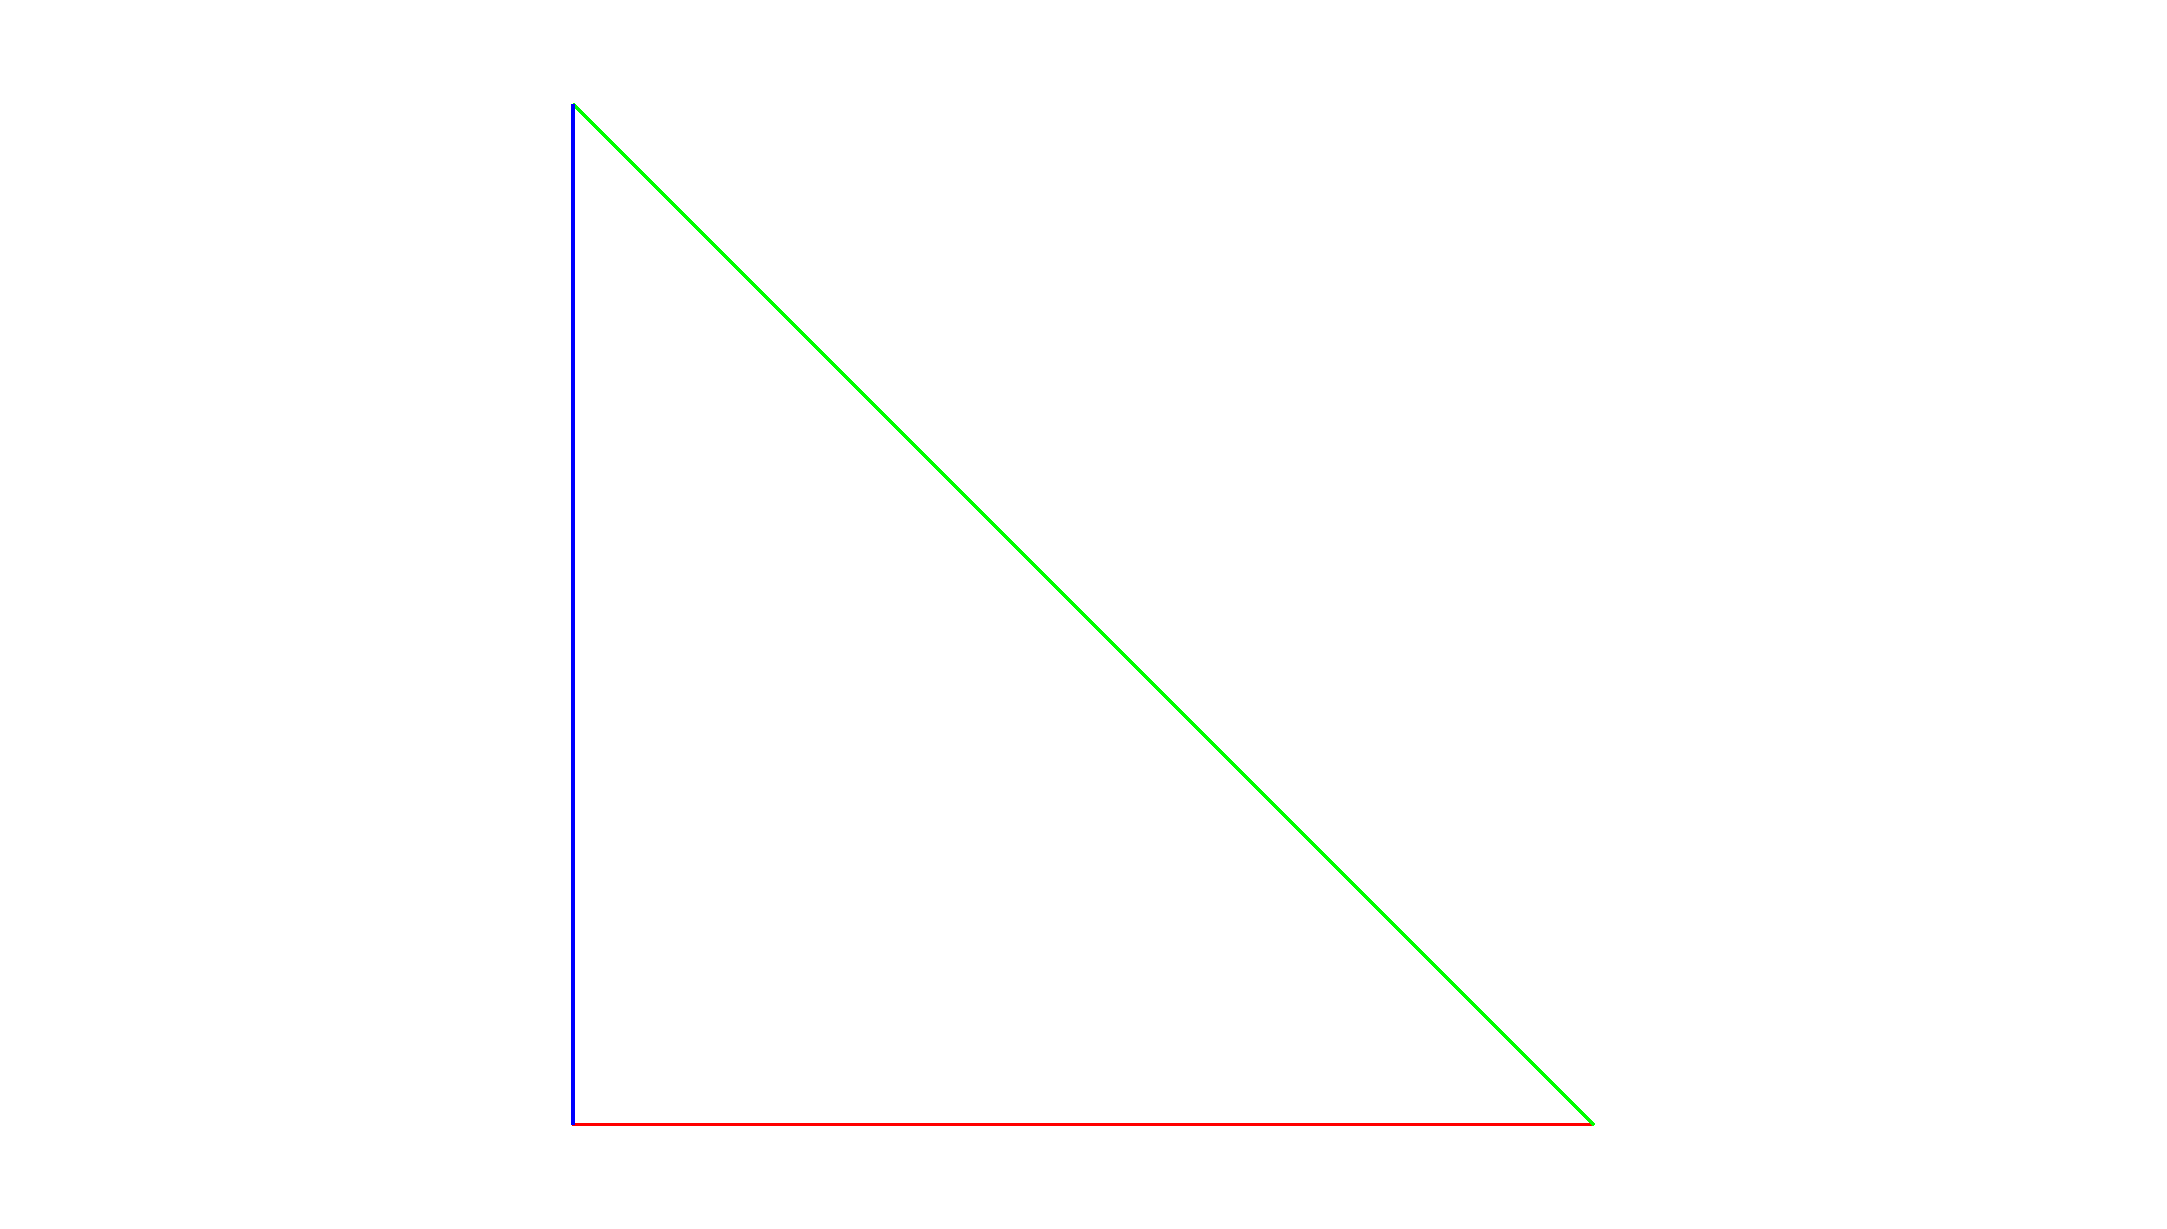
\includegraphics[width=6cm]{images/spiral-000}
  \end{latexonly}
  \begin{htmlonly}
    \htmladdimg{../images/spiral-000.png}
  \end{htmlonly}  
  \caption{The basic Formex}
\end{figure}

This basic Formex is copied 'm' times in the 0-direction with a translation 
step of '1' (the length of an edge of the triangle). After that, the new 
Formex is copied 'n' times in the 1-direction with a translation step of '1'. 
Because of the recursive definition (F=F.replic), the original Formex F is 
overwritten by the transformed one.
\begin{verbatim}
F = F.replic(m,1,0); drawit(F)
F = F.replic(n,1,1); drawit(F)
\end{verbatim}

Now a copy of this last Formex is translated in direction '2' with a 
translation step of '1'. This necessary for the transformation into a cilinder.
The result of all previous steps is a rectangular pattern with the desired 
dimensions, in a plane z=1.
\begin{verbatim}
F = F.translate(2,1); drawit(F,'iso')
\end{verbatim}
\begin{figure}[h]
  \centering
  \begin{makeimage}
  \end{makeimage}
  \begin{latexonly}
    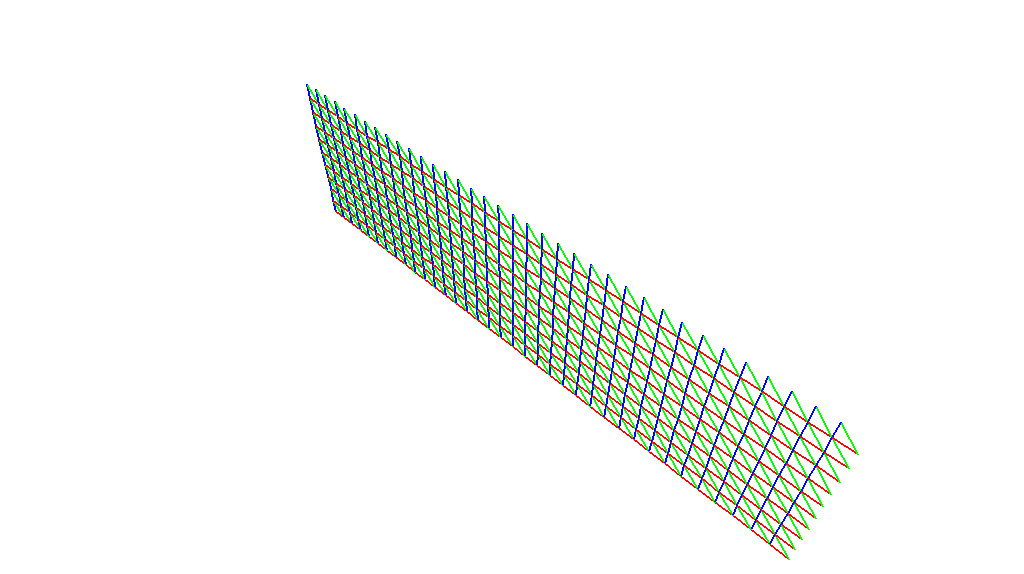
\includegraphics[width=6cm]{images/spiral-003}
  \end{latexonly}
  \begin{htmlonly}
    \htmladdimg{../images/spiral-003.png}
  \end{htmlonly}  
  \caption{The rectangular pattern}
\end{figure}

This pattern is rolled up into a cilinder around the 2-axis. 
\begin{verbatim}
F = F.cylindrical([2,1,0],[1.,360./n,1.]); drawit(F,'iso')
\end{verbatim}
\begin{figure}[h]
  \centering
  \begin{makeimage}
  \end{makeimage}
  \begin{latexonly}
    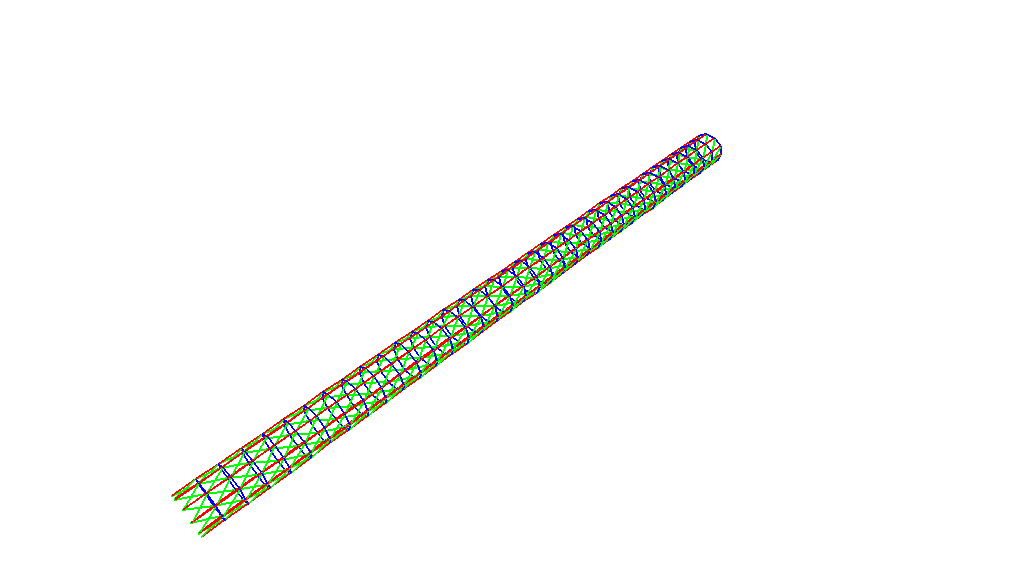
\includegraphics[width=6cm]{images/spiral-004}
  \end{latexonly}
  \begin{htmlonly}
    \htmladdimg{../images/spiral-004.png}
  \end{htmlonly}  
  \caption{The cylinder}
\end{figure}

This cilinder is copied 5 times in the 2-direction with a translation step of 
'm' (the lenght of the cilinder). 
\begin{verbatim}
F = F.replic(5,m,2); drawit(F,'iso')
\end{verbatim}

The next step is to rotate this cilinder -10 degrees around the 0-axis. 
This will determine the pitch angle of the spiral.
\begin{verbatim}
F = F.rotate(-10,0); drawit(F,'iso')
\end{verbatim}
\begin{figure}[h]
  \centering
  \begin{makeimage}
  \end{makeimage}
  \begin{latexonly}
    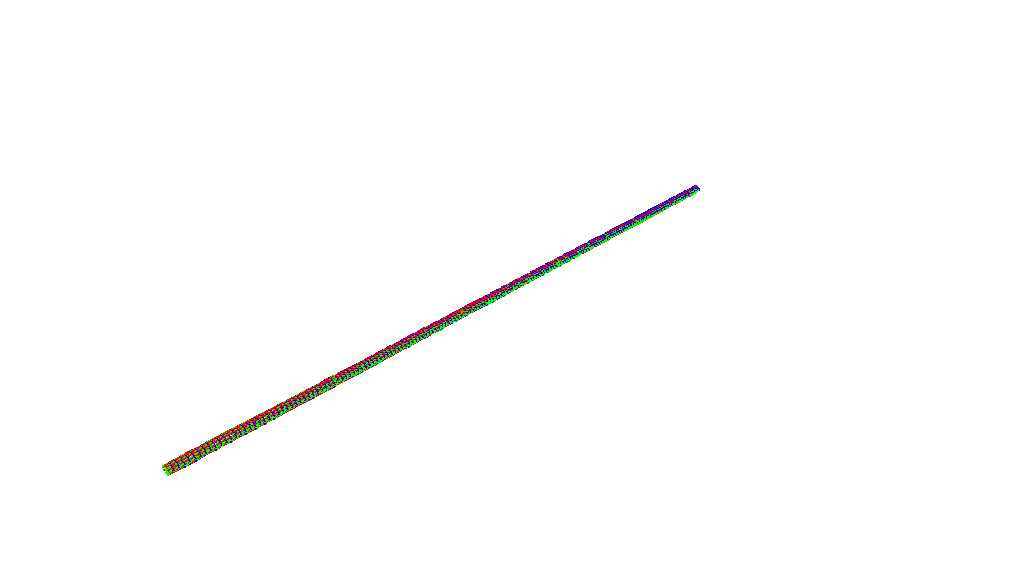
\includegraphics[width=6cm]{images/spiral-006}
  \end{latexonly}
  \begin{htmlonly}
    \htmladdimg{../images/spiral-006.png}
  \end{htmlonly}  
  \caption{The new cylinder}
\end{figure}

This last Formex is now translated in direction '0' with a translation step of '5'. 
\begin{verbatim}
F = F.translate(0,5); drawit(F,'iso')
\end{verbatim}

Finally, the Formex is rolled up, but around a different axis then before. 
Due to the pitch angle, a spiral is created. If the pitch angle would be 0 
(no rotation of -10 degrees around the 0-axis), the resulting Formex 
would be a torus. 
\begin{verbatim}
F = F.cylindrical([0,2,1],[1.,360./m,1.]); drawit(F,'iso')
drawit(F,'right')
\end{verbatim}
 \begin{figure}[h]
   \centering
   \begin{makeimage}
   \end{makeimage}
   \begin{latexonly}
     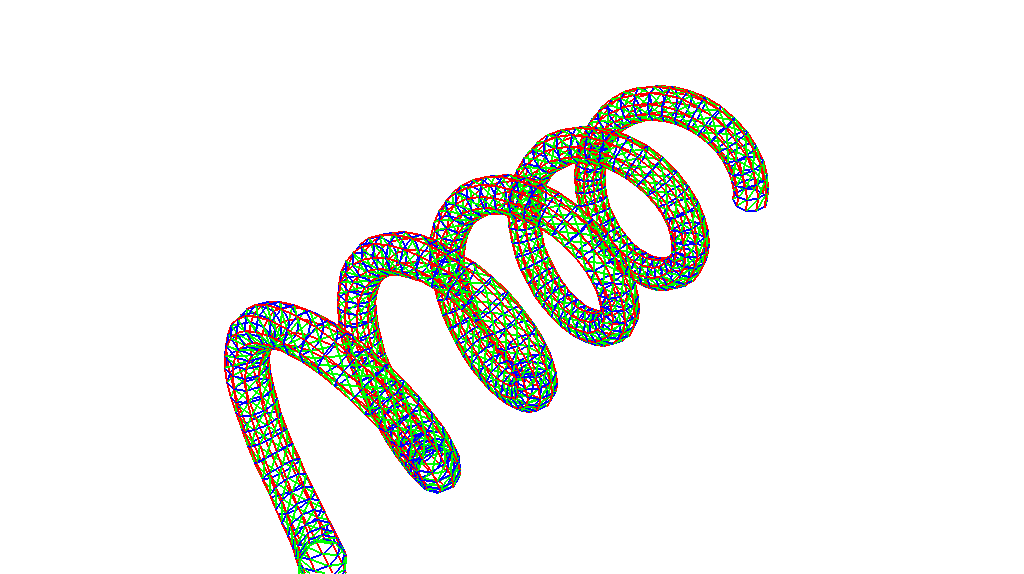
\includegraphics[width=5cm]{images/spiral-007}
     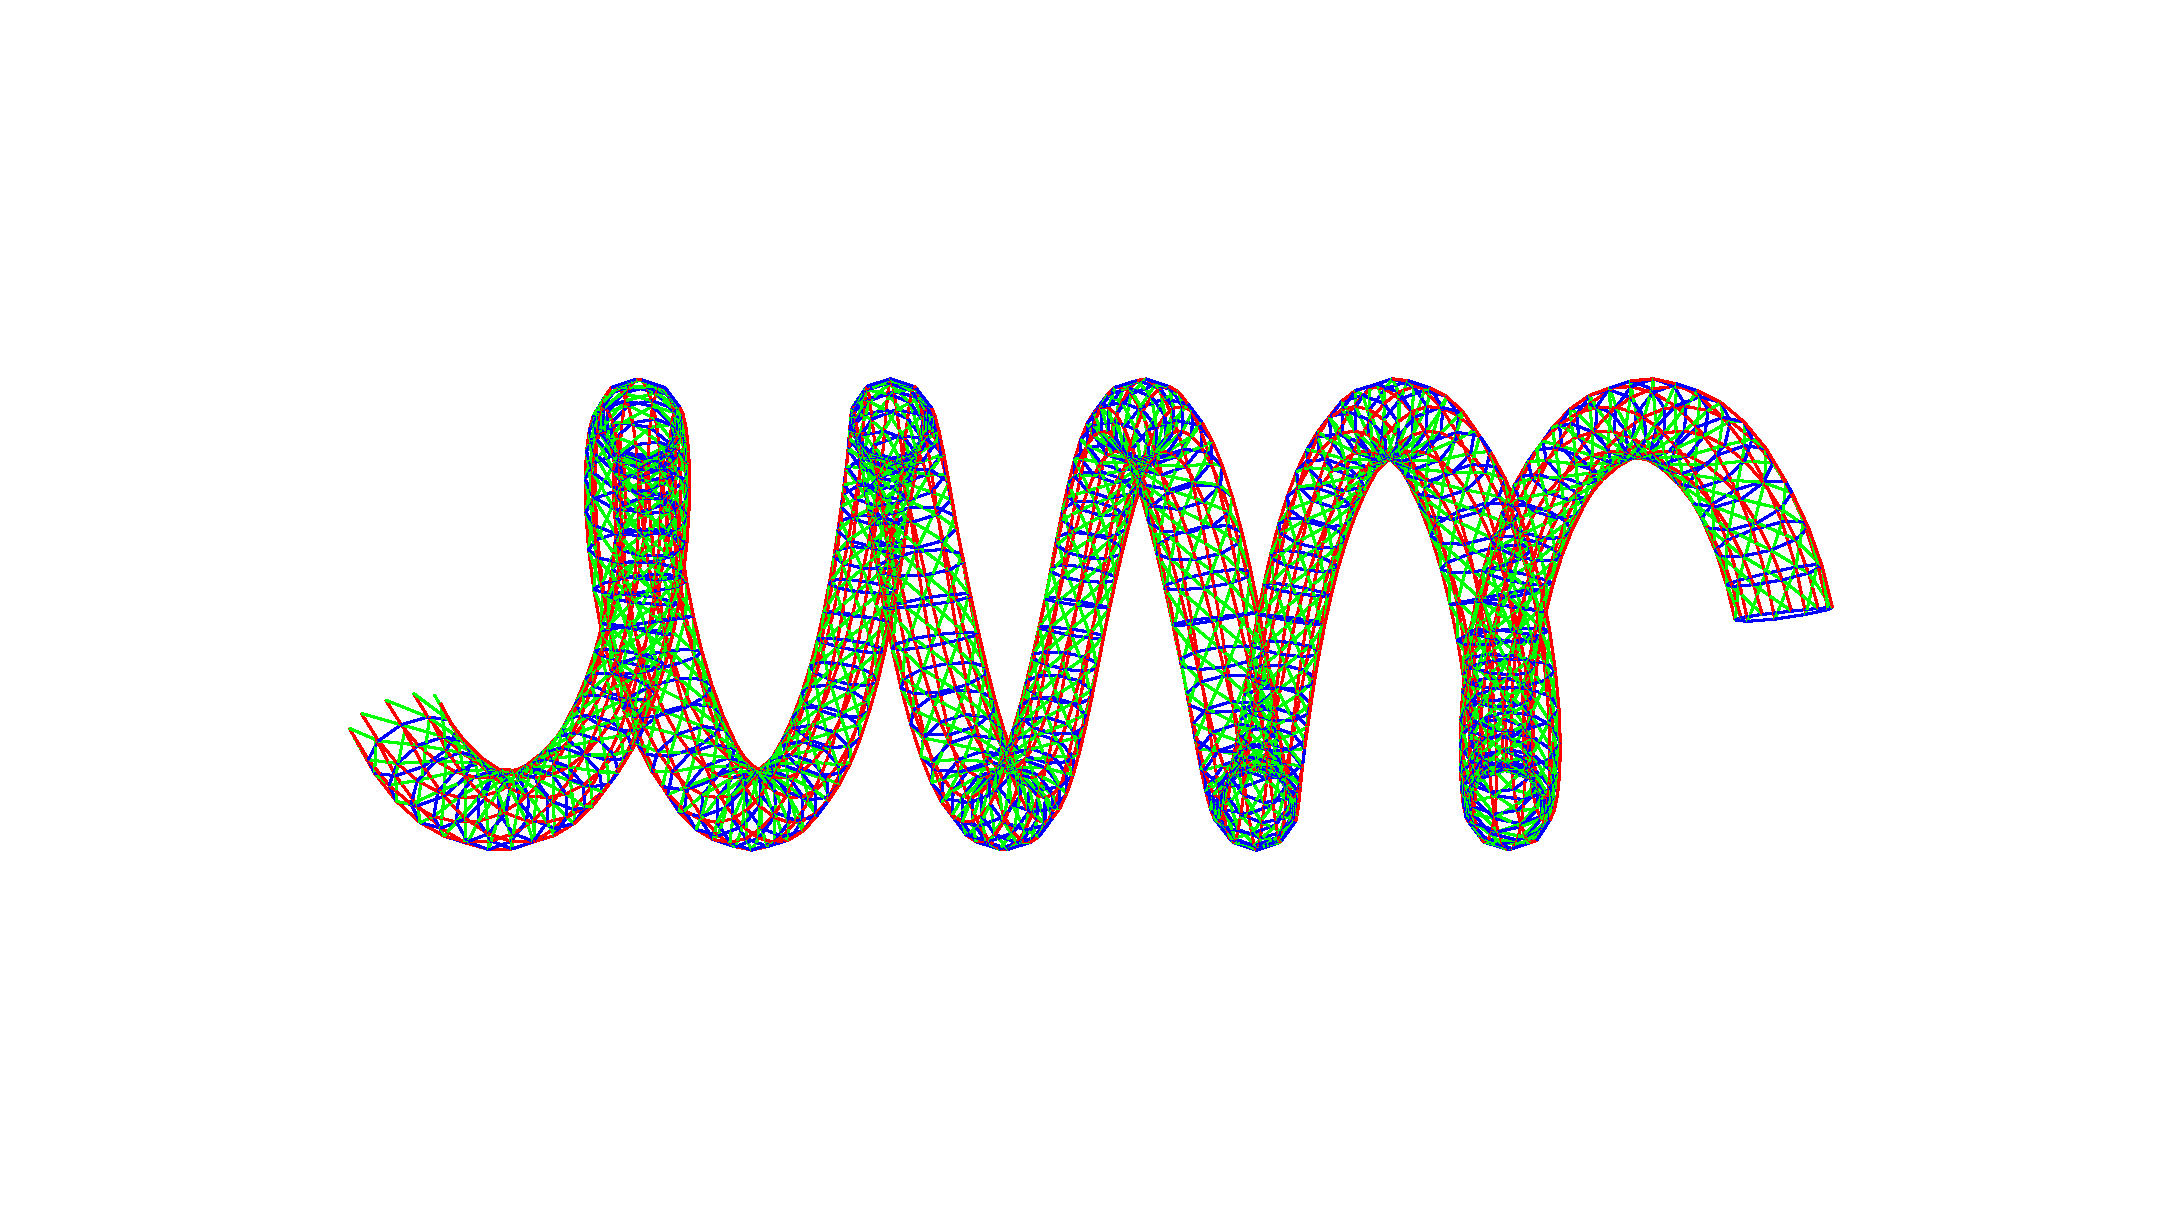
\includegraphics[width=5cm]{images/spiral-008}
   \end{latexonly}
   \begin{htmlonly}
     \htmladdimg{../images/spiral-007.png}
     \htmladdimg{../images/spiral-008.png}
   \end{htmlonly}  
   \caption{The spiral}
 \end{figure}

%%%%%%%%%%%%%%%%%%%%%%%%%%%%%%%%%%%%%%%%%%%%%%%%%%%%%%%%%%%%%%%%%
\section{Adding properties}
\label{sec:props}
Each element of a Formex can hold a property number. This number can be used as an entry in a database, which holds some sort of property. The module \module{properties} delivers such databases. The Formex and the database are seperate entities, only linked by the property numbers. 

\subsection{The class Property}
The first kind of database is called \class{Property}. This is the base class, and can hold any kind of property.
\begin{verbatim}
>>> Stick = Property(1, {'colour':'green', 'name':'Stick', 'weight': 25, 
'comment':'This could be anything: a gum, a frog, a usb-stick,...'})
>>> author = Property(5,{'Name':'Tim Neels', 'Address': CascadingDict
{'street':'Krijgslaan','city':'Gent','country':'Belgium'})})
\end{verbatim}
Data can be accessed in two ways: through the Property-instance itself, or through a dict 'properties'. 
\begin{verbatim}    
>>> print Stick
>>> print properties[1] 

  comment = This could be anything: a gum, a frog, a usb-stick,...
  colour = green
  name = Stick
  weight = 25

  comment = This could be anything: a gum, a frog, a usb-stick,...
  colour = green
  name = Stick
  weight = 25
\end{verbatim}
Adding and changing properties is very easy.
\begin{verbatim}  
>>> Stick.weight=30
>>> Stick.length=10
>>> print properties[1]

  comment = This could be anything: a gum, a frog, a usb-stick,...
  length = 10
  colour = green
  name = Stick
  weight = 30
\end{verbatim}

\subsection{The class NodeProperty}
The class NodeProperty can hold properties of nodes in finite element processing. The data is stored in a Dict called 'nodeproperties'. A NodeProperty can hold following sub-properties:
 \begin{description}
 \item [cload] A concentrated load. This is a list of 6 items
 \Code{[F_0, F_1, F_2, M_0, M_1, M_2]}. 
 \item [bound] A boundary condition. This can be defined in 2 ways:
     \begin{itemize}
     \item as a list of 6 items \Code{[ R_0, R_1, R_2, M_0, M_1, M_2 ]}. These items have 2 possible values:
         \begin{description}
         \item [0] The degree of freedom is not restrained.
         \item [1] The degree of freedom is restrained.
         \end{description}
     \item as a string. This string is a standard boundary type. In Abaqus several types are available:
         \begin{itemize}
         \item PINNED 
         \item ENCASTRE
         \item XSYMM
         \item YSYMM
         \item ZSYMM
         \item XASYMM
         \item YASYMM 
         \item ZASYMM
         \end{itemize} 
     \end{itemize}
 \item [displacement] The prescribed displacement. 
 \item [coords] The coordinate system which is used for the definition of cload and bound. There are three options:
         cartesian, spherical and cylindrical.
 \item [coordset] A list of 6 coordinates of the 2 points that specify the transformation: \Code{[x_1, y_1, z_1, x_2, y_2, z_2]}.
\end{description}

\begin{verbatim}
>>> top = NodeProperty(1,cload=[5,0,-75,0,0,0])
>>> foot = NodeProperty(2,bound='pinned')
>>> print 'nodeproperties'    
>>> for key, item in nodeproperties.iteritems():
>>>     print key, item

nodeproperties
1
  cload = [5, 0, -75, 0, 0, 0]
  coords = cartesian
  displacement = None
  bound = None
  coordset = []
2
  cload = None
  coords = cartesian
  displacement = None
  bound = pinned
  coordset = []
\end{verbatim}

\subsection{The class ElemProperty}
The class ElemProperty holds properties related to a single element. The data is stored in a Dict called 'elemproperties'. An element property can hold the following sub-properties:
\begin{description}
\item [elemsection] The section properties of the element. This is an ElemSection instance.
\item [elemload] The loading of the element. This is a list of ElemLoad instances.
\item [elemtype] The type of element that is to be used in the analysis. 
\end{description}

An elemsection can hold the following sub-properties:
\begin{description}
\item [section] The section properties of the element. This can be a dictionary or a string. The required data in this dict depends on the sectiontype. 
\item [material] The element material properties. This can be a dictionary which holds these properties or a string which can be used to search a material database. 
\item [sectiontype] The sectiontype of the element. 
\item [orientation]  A list [First direction cosine, second direction cosine, third direction cosine] of the first beam section axis. This allows to change the orientation of the cross-section.
\end{description}

An element load can hold the following sub-properties:
\begin{description}
\item [magnitude] The magnitude of the distibuted load.
\item [loadlabel] The distributed load type label.
\end{description}

The general structure of the element properties database looks like this:
\begin{itemize}
\item[-] Property
\item[-] NodeProperty
    \begin{itemize}
    \item[-] cload
    \item[-] bound
    \item[-] displacement
    \item[-] coords
    \item[-] coordset
    \end{itemize}
\item[-] ElemProperty 
    \begin{itemize}
    \item[-] elemsection
        \begin{itemize}
        \item[-] section
        \item[-] material
        \item[-] sectiontype
        \item[-] orientation
        \end{itemize}
    \item[-] elemload
        \begin{itemize}
        \item[-] magnitude
        \item[-] loadlabel
        \end{itemize}
    \item[-] elemtype
    \end{itemize}
\end{itemize}

\begin{verbatim}
>>> vert = ElemSection('IPEA100', 'steel')
>>> hor = ElemSection({'name':'IPEM800','A':951247,'I':CascadingDict(
{'Ix':1542,'Iy':6251,'Ixy':352})}, {'name':'S400','E':210,'fy':400})
>>> q = ElemLoad(magnitude=2.5, loadlabel='PZ')
>>> top = ElemProperty(1,hor,[q],'B22')
>>> column = ElemProperty(2,vert, elemtype='B22')
>>> diagonal = ElemProperty(4,hor,elemtype='B22')

>>> print 'elemproperties'
>>> for key, item in elemproperties.iteritems():
>>>     print key, item    

elemproperties
1
  elemtype = B22
  elemload = [CascadingDict({'magnitude': 2.5, 'loadlabel': 'PZ'})]
  elemsection =
    section =
      A = 951247
      I =
        Iy = 6251
        Ix = 1542
        Ixy = 352
      name = IPEM800
    material =
      fy = 400
      E = 210
      name = S400
    orientation = None
    sectiontype = general
2
  elemtype = B22
  elemload = None
  elemsection =
    section =
      torsional_rigidity = 1542
      name = IPEA100
      moment_inertia_22 = 1140000
      cross_section = 878
      moment_inertia_11 = 1412000
      moment_inertia_12 = 1254
    material =
      shear_modulus = 25
      young_modulus = 210
      name = steel
    orientation = None
    sectiontype = general
4
  elemtype = B22
  elemload = None
  elemsection =
    section =
      A = 951247
      I =
        Iy = 6251
        Ix = 1542
        Ixy = 352
      name = IPEM800
    material =
      fy = 400
      E = 210
      name = S400
    orientation = None
    sectiontype = general
\end{verbatim}


%
\section{Exporting to finite element programs}


%
%%% Local Variables: 
%%% mode: latex
%%% TeX-master: "manual"
%%% End: 
